\documentclass[tikz,border=2pt]{standalone}
\usepackage{tikz}
\usepackage[european]{circuitikz}
\usetikzlibrary{arrows.meta,positioning,calc}
../cictikz/src/cictikz/data/tex/cictikz_lib.tex
\begin{document}
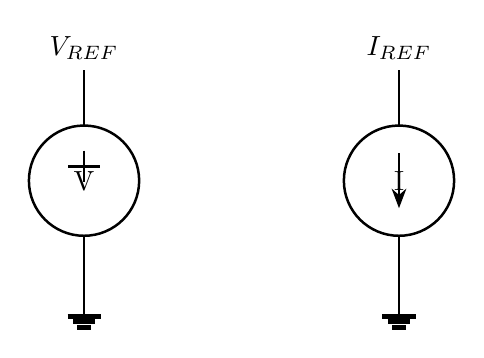
\begin{tikzpicture}[>=Stealth, line width=0.9pt]
  \draw (0,0) circle (0.7) node {V};
  \draw (0,-0.7) -- (0,-1.3) node[ground] {};
  \draw (0,0.7) -- (0,1.4) node[above] {$V_{REF}$};
  \draw (0.2,0.18) -- (-0.2,0.18);
  \draw (0,0.38) -- (0,-0.02);

  \draw (4,0) circle (0.7) node {I};
  \draw (4,-0.7) -- (4,-1.3) node[ground] {};
  \draw (4,0.7) -- (4,1.4) node[above] {$I_{REF}$};
  \draw[->] (4,0.35) -- (4,-0.35);
\end{tikzpicture}
\end{document}
